\scanpage{184}\mspage{39}%
% archive sheet number: 184
on arrive à réconstituer le type d'homotopie via son $\infty$-groupoïde fondamental, comme expliqué dans ma lettre précédente, \deleted{\unsure{e|a}}et rappelé dans celle-ci. (Cela signifie en particulier que toutes les opérations cohomologiques possibles et imaginables sont déjà incluses dans la donnée d'un tel système de $n$-catégories .\,.\,.\,.) \deleted{Mais}

De même, les types d'homotopie plus \unsure{cannelés|canelés}, liés à certains diagrammes finis, qu'on peut associer à \deleted{\unsure{des}}certains types de stratifications \inserted{$\unsure{\mathcal P|P}$} d'espaces topologiques ``modérés'' $X$ disons%
% Compact isolated point at (702,1186), above the latter part of disons; origin uncertain.
\raisebox{0pt}[0pt][0pt]{\parbox{0pt}{\figure{\begin{tikzpicture}[overlay,x=1em,y=1ex]\fill (-0.8,3.0) circle (0.35pt);\end{tikzpicture}}}}%
, devraient correspondre de façon aussi parfaite aux \deleted{\unsure{$n$-}}\inserted{$(n+1)$-}catégories%
% Isolated point at (1156,1367), below the g-descender of catégories; origin uncertain.
\raisebox{0pt}[0pt][0pt]{\parbox{0pt}{\figure{\begin{tikzpicture}[overlay,x=1em,y=1ex]\fill (-2.3,-2.0) circle (0.4pt);\end{tikzpicture}}}}
de $n$-champs sur $X$ qui sont loc \unsure{constant|constants} sur chacune des strates de $\mathcal P$ (disons: qui sont subordonnés à $\mathcal P$)%
% Separate compact point at (1622,1482), above/right of the closing parenthesis; origin uncertain.
\raisebox{0pt}[0pt][0pt]{\parbox{0pt}{\figure{\begin{tikzpicture}[overlay,x=1em,y=1ex]\fill (0,2.5) circle (0.35pt);\end{tikzpicture}}}}.
Si plus haut le topis de la cat. dérivée loc. constante marchait bel et bien, on s'attendrait ici à récupérer le type d'homotopie mixte à partir de la \inserted{ss-}%
% Curved insertion guide at the start of catégorie. Two separate points below it,
% at (1001,1963) and (996,1970), are reproduced without a punctuation interpretation.
\raisebox{0pt}[0pt][0pt]{\parbox{0pt}{\figure{\begin{tikzpicture}[overlay,x=1em,y=1ex]\draw[line width=0.35pt] (-0.12,-0.15) .. controls (-0.06,0.65) and (0.35,1.45) .. (0.76,1.65);\fill (-0.05,-2.55) circle (0.35pt);\fill (-0.15,-3.0) circle (0.35pt);\end{tikzpicture}}}}catégorie de la \unsure{catégori|catégorie} dérivée des faisceaux abéliens sur $X$, formée des complexes qui \unsure{sont|ont} \unsure{à|:} ch. loc. \unsure{constant|constante} sur chacune des strates -- avec en plus les opérations $\overset{\mathbb{L}}{\otimes}$, $\mathbb{R}\underline{\mathrm{Hom}}$ plus, \unsure{les|le}
